\section{Introduction}\label{introduction}

\begin{frame}{Good Quote}

\begin{quote}
``The commonality between science and art is in trying to see profoundly
- to develop strategies of seeing and showing.''

--- Edward Tufte
\end{quote}

\end{frame}

\begin{frame}[fragile]{Introduction}

Once again, we will turn to our friend \texttt{ggplot2} to plot; but
now, we are going to take it to another level. We will use many of the
options that this powerful package provides and discuss briefly some
important aspects of a good plot.

We will go through several aspects of the code that makes plotting in
\texttt{R} flexible and beautiful.

\begin{enumerate}
\def\labelenumi{\arabic{enumi}.}
\tightlist
\item
  Types of plots
\item
  Color schemes
\item
  Themes
\item
  Labels and titles
\item
  Facetting
\end{enumerate}

\end{frame}

\begin{frame}[fragile]{Introduction}

To highlight these features we'll be using our NHANES data again;
specifically, sedentary behavior, depression, asthma, family size, and
race. As this is only an introduction, refer to
\url{http://docs.ggplot2.org/current/} for more information on
\texttt{ggplot2}.

\end{frame}

\begin{frame}[fragile]{Introduction}

To begin, it needs to be understood that the first line where we
actually use the \texttt{ggplot} function, will then apply to all
subsequent laters (e.g., \texttt{geom\_point()}). For example,

\begin{Shaded}
\begin{Highlighting}[]
\KeywordTok{ggplot}\NormalTok{(df, }\KeywordTok{aes}\NormalTok{(}\DataTypeTok{x =}\NormalTok{ dep, }\DataTypeTok{y =}\NormalTok{ sed, }\DataTypeTok{group =}\NormalTok{ asthma))}
\end{Highlighting}
\end{Shaded}

means for the rest of the layers, unless we over-ride it, each will use
\texttt{df} with \texttt{dep} as the x variable, \texttt{sed} as the y,
and a grouping on \texttt{asthma}. So when many layers are going to use
the same command put it in this so you don't have to write the same
argument many times. A common one here could be:

\begin{Shaded}
\begin{Highlighting}[]
\KeywordTok{ggplot}\NormalTok{(df, }\KeywordTok{aes}\NormalTok{(}\DataTypeTok{x =}\NormalTok{ dep, }\DataTypeTok{y =}\NormalTok{ sed, }
               \DataTypeTok{group =}\NormalTok{ asthma, }
               \DataTypeTok{color =}\NormalTok{ asthma))}
\end{Highlighting}
\end{Shaded}

since we often want to color by our grouping variable.

\end{frame}

\begin{frame}[fragile]{Incomplete Plots}

Before going forward, a nice feature of \texttt{ggplot2} allows us to
use an ``incomplete'' plot to add on to. For example, if we have a good
idea of the main structure of the plot but want to explore some changes,
we can do the following:

\begin{Shaded}
\begin{Highlighting}[]
\NormalTok{p1 <-}\StringTok{ }\KeywordTok{ggplot}\NormalTok{(df, }\KeywordTok{aes}\NormalTok{(}\DataTypeTok{x =}\NormalTok{ dep, }\DataTypeTok{y =}\NormalTok{ sed, }\DataTypeTok{group =}\NormalTok{ asthma)) }\OperatorTok{+}
\StringTok{  }\KeywordTok{geom_point}\NormalTok{()}
\NormalTok{p1}
\end{Highlighting}
\end{Shaded}

\end{frame}

\begin{frame}[fragile]{Incomplete Plots}

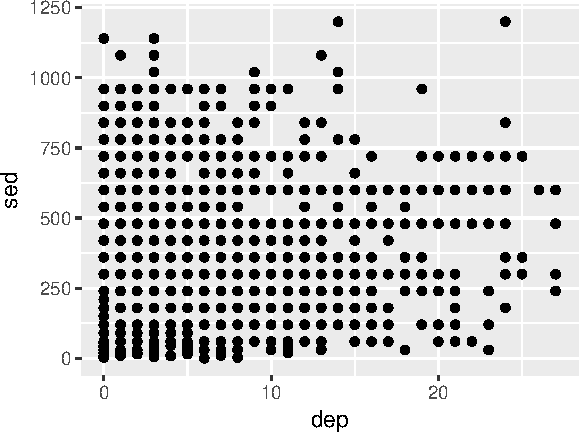
\includegraphics{09_AdvancedPlotting_files/figure-beamer/c1-1.pdf}

So now \texttt{p1} has the information for this basic, and honestly
fairly uninformative, plot. We'll use this feature to build on plots
that we like.

\end{frame}

\begin{frame}[fragile]{Data Prep}

Some of our figures will also need summary data so we'll start that here
as well:

\begin{Shaded}
\begin{Highlighting}[]
\NormalTok{summed_data <-}\StringTok{ }\NormalTok{df }\OperatorTok
\StringTok{  }\KeywordTok{group_by}\NormalTok{(asthma, dep2) }\OperatorTok
\StringTok{  }\KeywordTok{summarize}\NormalTok{(}\DataTypeTok{s_se =} \KeywordTok{sd}\NormalTok{(sed, }\DataTypeTok{na.rm=}\OtherTok{TRUE}\NormalTok{)}\OperatorTok{/}\KeywordTok{sqrt}\NormalTok{(}\KeywordTok{n}\NormalTok{()),}
            \DataTypeTok{sed  =} \KeywordTok{mean}\NormalTok{(sed, }\DataTypeTok{na.rm=}\OtherTok{TRUE}\NormalTok{),}
            \DataTypeTok{N    =} \KeywordTok{n}\NormalTok{())}
\end{Highlighting}
\end{Shaded}

As you hopefully recognize a bit, we are summarizing the time spent
being sedentary by both asthma and the dichotomous depression variables.
If it doesn't make sense at first, read it line by line to see what I
did. This will be useful for several types of plots.

\end{frame}

\section{Types of Plots}\label{types-of-plots}

\begin{frame}[fragile]{Scatterplots}

We'll start with a scatterplot--one of the most simple yet informative
plots.

\begin{Shaded}
\begin{Highlighting}[]
\KeywordTok{ggplot}\NormalTok{(df, }\KeywordTok{aes}\NormalTok{(}\DataTypeTok{x =}\NormalTok{ dep, }\DataTypeTok{y =}\NormalTok{ sed, }
               \DataTypeTok{group =}\NormalTok{ asthma)) }\OperatorTok{+}
\StringTok{  }\KeywordTok{geom_point}\NormalTok{(}\KeywordTok{aes}\NormalTok{(}\DataTypeTok{color =}\NormalTok{ asthma))}
\end{Highlighting}
\end{Shaded}

\end{frame}

\begin{frame}{Scatterplots}

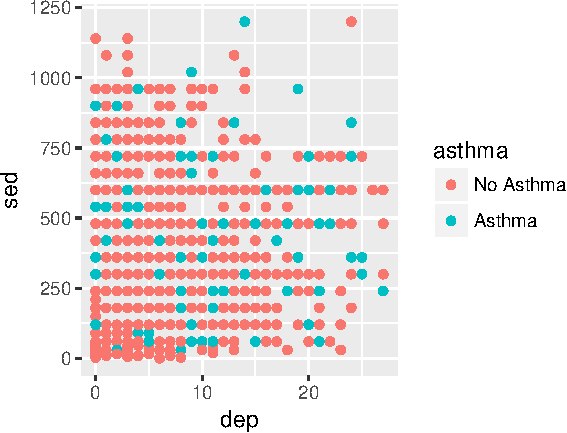
\includegraphics{09_AdvancedPlotting_files/figure-beamer/c2-1.pdf}

\end{frame}

\begin{frame}[fragile]{Scatterplots}

It's not amazing. There looks to be a lot of overlap of the points.
Also, it would be nice to know general trend lines for each group.
Below, \texttt{alpha} refers to how transparent the points are,
\texttt{method\ =\ "lm"} refers to how the line should be fit, and
\texttt{se=FALSE} tells it not to include error ribbons.

\begin{Shaded}
\begin{Highlighting}[]
\KeywordTok{ggplot}\NormalTok{(df, }\KeywordTok{aes}\NormalTok{(}\DataTypeTok{x =}\NormalTok{ dep, }\DataTypeTok{y =}\NormalTok{ sed, }\DataTypeTok{group =}\NormalTok{ asthma)) }\OperatorTok{+}
\StringTok{  }\KeywordTok{geom_jitter}\NormalTok{(}\KeywordTok{aes}\NormalTok{(}\DataTypeTok{color =}\NormalTok{ asthma), }\DataTypeTok{alpha =}\NormalTok{ .}\DecValTok{5}\NormalTok{) }\OperatorTok{+}
\StringTok{  }\KeywordTok{geom_smooth}\NormalTok{(}\KeywordTok{aes}\NormalTok{(}\DataTypeTok{color =}\NormalTok{ asthma), }
              \DataTypeTok{method =} \StringTok{"lm"}\NormalTok{, }\DataTypeTok{se=}\OtherTok{FALSE}\NormalTok{)}
\end{Highlighting}
\end{Shaded}

\end{frame}

\begin{frame}{Scatterplots}

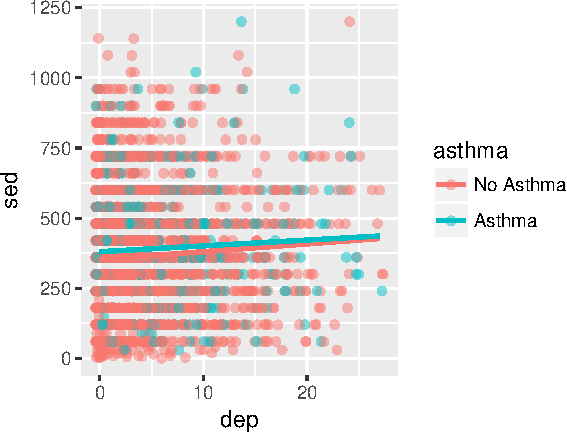
\includegraphics{09_AdvancedPlotting_files/figure-beamer/c3-1.pdf}

\end{frame}

\begin{frame}{Scatterplots}

It's getting better but we could still use some more features. We'll
come back to this in the next sections.

\end{frame}

\begin{frame}[fragile]{Boxplots}

Box plots are great ways to assess the variability in your data. Below,
we create a boxplot but change \texttt{p1}'s x variable so that it is
the factor version of depression.

\begin{Shaded}
\begin{Highlighting}[]
\KeywordTok{ggplot}\NormalTok{(df, }\KeywordTok{aes}\NormalTok{(}\DataTypeTok{x =} \KeywordTok{factor}\NormalTok{(dep2), }\DataTypeTok{y =}\NormalTok{ sed)) }\OperatorTok{+}
\StringTok{  }\KeywordTok{geom_boxplot}\NormalTok{()}
\end{Highlighting}
\end{Shaded}

\end{frame}

\begin{frame}{Boxplots}

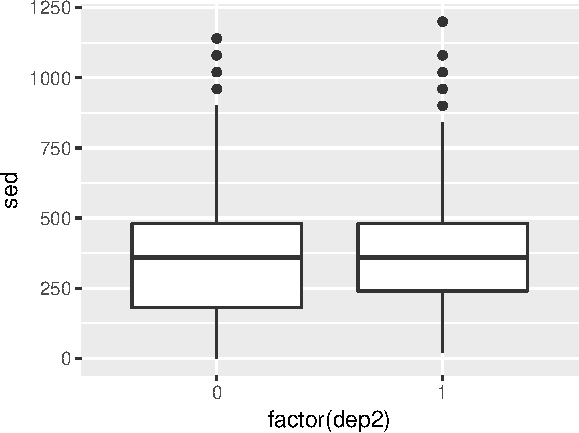
\includegraphics{09_AdvancedPlotting_files/figure-beamer/c4-1.pdf}

\end{frame}

\begin{frame}[fragile]{Boxplots}

This plot is, at best, mediocre. But there's more we can do.

\begin{Shaded}
\begin{Highlighting}[]
\KeywordTok{ggplot}\NormalTok{(df, }\KeywordTok{aes}\NormalTok{(}\DataTypeTok{x =} \KeywordTok{factor}\NormalTok{(dep2), }\DataTypeTok{y =} \KeywordTok{jitter}\NormalTok{(sed, }\DecValTok{100}\NormalTok{))) }\OperatorTok{+}
\StringTok{  }\KeywordTok{geom_jitter}\NormalTok{(}\DataTypeTok{alpha =}\NormalTok{ .}\DecValTok{1}\NormalTok{, }\DataTypeTok{color =} \StringTok{"chartreuse4"}\NormalTok{) }\OperatorTok{+}
\StringTok{  }\KeywordTok{geom_boxplot}\NormalTok{(}\DataTypeTok{alpha =}\NormalTok{ .}\DecValTok{75}\NormalTok{, }\DataTypeTok{color =} \StringTok{"dodgerblue4"}\NormalTok{) }
\end{Highlighting}
\end{Shaded}

\end{frame}

\begin{frame}{Boxplots}

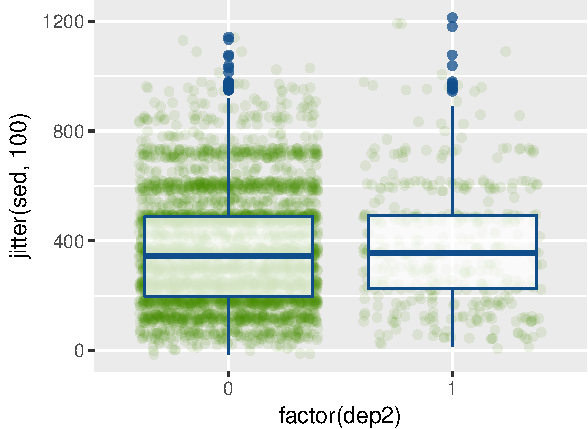
\includegraphics{09_AdvancedPlotting_files/figure-beamer/c5-1.pdf}

\end{frame}

\begin{frame}{Boxplots}

This now provides the (jittered) raw data points as well to hightlight
the noise and the number of observations in each group.

\end{frame}

\begin{frame}[fragile]{Bar Plots}

Bar plots are great ways to look at means and standard deviations for
groups.

\begin{Shaded}
\begin{Highlighting}[]
\KeywordTok{ggplot}\NormalTok{(summed_data, }\KeywordTok{aes}\NormalTok{(}\DataTypeTok{x =}\NormalTok{ dep2, }\DataTypeTok{y =}\NormalTok{ sed, }
                        \DataTypeTok{group =}\NormalTok{ asthma)) }\OperatorTok{+}
\StringTok{  }\KeywordTok{geom_bar}\NormalTok{(}\KeywordTok{aes}\NormalTok{(}\DataTypeTok{fill =}\NormalTok{ asthma), }
           \DataTypeTok{stat =} \StringTok{"identity"}\NormalTok{, }
           \DataTypeTok{position =} \StringTok{"dodge"}\NormalTok{)}
\end{Highlighting}
\end{Shaded}

\end{frame}

\begin{frame}{Bar Plots}

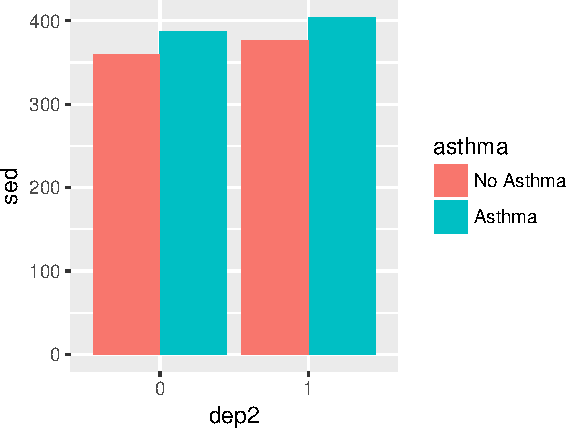
\includegraphics{09_AdvancedPlotting_files/figure-beamer/c6-1.pdf}

\end{frame}

\begin{frame}[fragile]{Bar Plots}

We used \texttt{stat\ =\ "identity"} to make it based on the mean
(default is \texttt{count}), and \texttt{position\ =\ "dodge"} makes it
so the bars are next to each other as opposed to stacked. Let's also add
error bars.

\end{frame}

\begin{frame}[fragile]{Bar Plots}

\begin{Shaded}
\begin{Highlighting}[]
\NormalTok{p =}\StringTok{ }\KeywordTok{position_dodge}\NormalTok{(}\DataTypeTok{width =}\NormalTok{ .}\DecValTok{9}\NormalTok{)}
\KeywordTok{ggplot}\NormalTok{(summed_data, }\KeywordTok{aes}\NormalTok{(}\DataTypeTok{x =}\NormalTok{ dep2, }\DataTypeTok{y =}\NormalTok{ sed, }
                        \DataTypeTok{group =}\NormalTok{ asthma)) }\OperatorTok{+}
\StringTok{  }\KeywordTok{geom_bar}\NormalTok{(}\KeywordTok{aes}\NormalTok{(}\DataTypeTok{fill =}\NormalTok{ asthma), }
           \DataTypeTok{stat =} \StringTok{"identity"}\NormalTok{, }
           \DataTypeTok{position =}\NormalTok{ p,}
           \DataTypeTok{alpha =}\NormalTok{ .}\DecValTok{8}\NormalTok{) }\OperatorTok{+}
\StringTok{  }\KeywordTok{geom_errorbar}\NormalTok{(}\KeywordTok{aes}\NormalTok{(}\DataTypeTok{ymin =}\NormalTok{ sed }\OperatorTok{-}\StringTok{ }\NormalTok{s_se, }\DataTypeTok{ymax =}\NormalTok{ sed }\OperatorTok{+}\StringTok{ }\NormalTok{s_se,}
                    \DataTypeTok{color =}\NormalTok{ asthma), }
                \DataTypeTok{position =}\NormalTok{ p,}
                \DataTypeTok{width =}\NormalTok{ .}\DecValTok{3}\NormalTok{)}
\end{Highlighting}
\end{Shaded}

\end{frame}

\begin{frame}{Bar Plots}

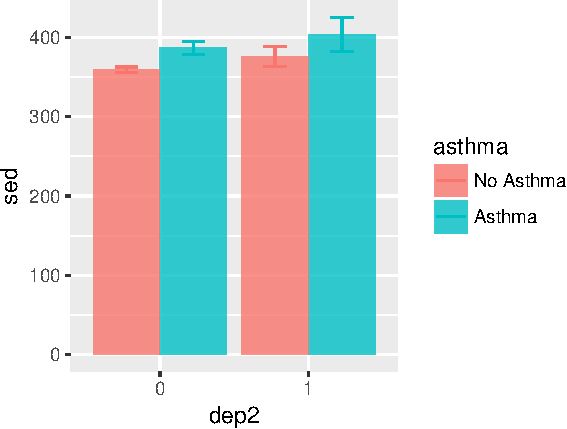
\includegraphics{09_AdvancedPlotting_files/figure-beamer/c7-1.pdf}

\end{frame}

\begin{frame}[fragile]{Bar Plots}

There's a lot in there but much of it is what you've seen before. For
example, we use \texttt{alpha} in the \texttt{geom\_bar()} to tell it to
be slightly transparent so we can see the error bars better. We used the
\texttt{position\_dodge()} function to specify exactly how much dodge we
wanted. In this way, we are able to line up the error bars and the bars.
If we just use \texttt{position\ =\ "dodge"} we have less flexibility
and control.

Much more can be done to clean this up, which we'll show in later
sections.

\end{frame}

\begin{frame}[fragile]{Line Plots}

Line plots are particularly good at showing trends and relationships.
Below we we use it to highlight the relationship between depression,
sedentary behavior, and asthma.

\begin{Shaded}
\begin{Highlighting}[]
\KeywordTok{ggplot}\NormalTok{(summed_data, }\KeywordTok{aes}\NormalTok{(}\DataTypeTok{x =}\NormalTok{ dep2, }\DataTypeTok{y =}\NormalTok{ sed, }
                        \DataTypeTok{group =}\NormalTok{ asthma)) }\OperatorTok{+}
\StringTok{  }\KeywordTok{geom_line}\NormalTok{(}\KeywordTok{aes}\NormalTok{(}\DataTypeTok{color =}\NormalTok{ asthma))}
\end{Highlighting}
\end{Shaded}

\end{frame}

\begin{frame}{Line Plots}

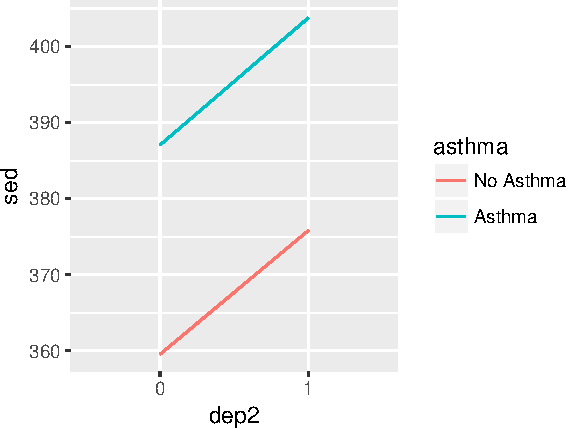
\includegraphics{09_AdvancedPlotting_files/figure-beamer/c8-1.pdf}

\end{frame}

\begin{frame}[fragile]{Line Plots}

Good start, but let's add some features.

\begin{Shaded}
\begin{Highlighting}[]
\NormalTok{pos =}\StringTok{ }\KeywordTok{position_dodge}\NormalTok{(}\DataTypeTok{width =}\NormalTok{ .}\DecValTok{1}\NormalTok{)}
\KeywordTok{ggplot}\NormalTok{(summed_data, }\KeywordTok{aes}\NormalTok{(}\DataTypeTok{x =}\NormalTok{ dep2, }\DataTypeTok{y =}\NormalTok{ sed, }
                        \DataTypeTok{group =}\NormalTok{ asthma, }
                        \DataTypeTok{color =}\NormalTok{ asthma)) }\OperatorTok{+}
\StringTok{  }\KeywordTok{geom_line}\NormalTok{(}\DataTypeTok{position =}\NormalTok{ pos) }\OperatorTok{+}
\StringTok{  }\KeywordTok{geom_point}\NormalTok{(}\DataTypeTok{position =}\NormalTok{ pos) }\OperatorTok{+}
\StringTok{  }\KeywordTok{geom_errorbar}\NormalTok{(}\KeywordTok{aes}\NormalTok{(}\DataTypeTok{ymin =}\NormalTok{ sed }\OperatorTok{-}\StringTok{ }\NormalTok{s_se, }
                    \DataTypeTok{ymax =}\NormalTok{ sed }\OperatorTok{+}\StringTok{ }\NormalTok{s_se), }
                \DataTypeTok{width =}\NormalTok{ .}\DecValTok{1}\NormalTok{, }
                \DataTypeTok{position =}\NormalTok{ pos)}
\end{Highlighting}
\end{Shaded}

\end{frame}

\begin{frame}{Line Plots}

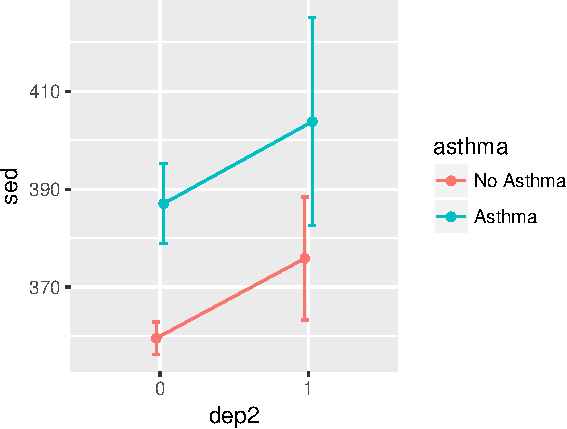
\includegraphics{09_AdvancedPlotting_files/figure-beamer/c9-1.pdf}

That looks a bit better. From here, let's go on to color schemes to make
the plots a bit better.

\end{frame}

\section{Color Schemes}\label{color-schemes}

\begin{frame}[fragile]{Color Schemes}

We'll start by using the scatterplot we made above but we will change
the colors a bit using \texttt{scale\_color\_manual()}.

\begin{Shaded}
\begin{Highlighting}[]
\KeywordTok{ggplot}\NormalTok{(df, }\KeywordTok{aes}\NormalTok{(}\DataTypeTok{x =}\NormalTok{ dep, }\DataTypeTok{y =}\NormalTok{ sed, }\DataTypeTok{group =}\NormalTok{ asthma)) }\OperatorTok{+}
\StringTok{  }\KeywordTok{geom_jitter}\NormalTok{(}\KeywordTok{aes}\NormalTok{(}\DataTypeTok{color =}\NormalTok{ asthma), }\DataTypeTok{alpha =}\NormalTok{ .}\DecValTok{5}\NormalTok{) }\OperatorTok{+}
\StringTok{  }\KeywordTok{geom_smooth}\NormalTok{(}\KeywordTok{aes}\NormalTok{(}\DataTypeTok{color =}\NormalTok{ asthma), }
              \DataTypeTok{method =} \StringTok{"lm"}\NormalTok{, }\DataTypeTok{se=}\OtherTok{FALSE}\NormalTok{) }\OperatorTok{+}
\StringTok{  }\KeywordTok{scale_color_manual}\NormalTok{(}\DataTypeTok{values =} \KeywordTok{c}\NormalTok{(}\StringTok{"dodgerblue4"}\NormalTok{, }
                                \StringTok{"chartreuse4"}\NormalTok{))}
\end{Highlighting}
\end{Shaded}

\end{frame}

\begin{frame}[fragile]{Color Schemes}

We'll start by using the scatterplot we made above but we will change
the colors a bit using \texttt{scale\_color\_manual()}.
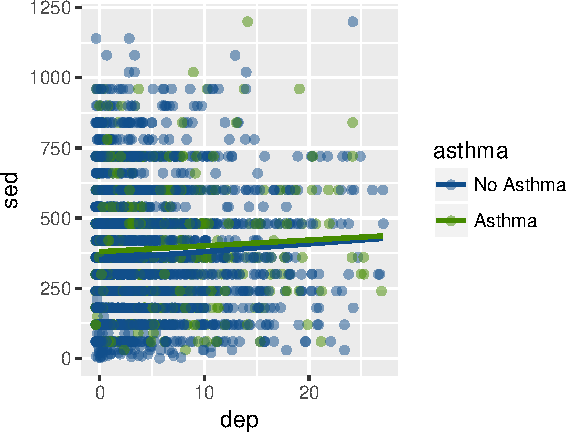
\includegraphics{09_AdvancedPlotting_files/figure-beamer/cs2-1.pdf}

\end{frame}

\begin{frame}{Color Schemes}

\begin{quote}
Don't get too lost in selecting colors but it can add a nice touch to
any plot. The nuances of plot design can be invigorating but also time
consuming to be smart about how long you spend using it.
\end{quote}

Next, let's adjust the bar plot. We will also add some colors here, but
we will differentiate between ``color'' and ``fill''.

\begin{enumerate}
\def\labelenumi{\arabic{enumi}.}
\tightlist
\item
  Fill fills in the object with color. This is useful for things that
  are more than simply a line or a dot.
\item
  Color colors the object. This outlines those items that can also be
  filled and colors lines and dots.
\end{enumerate}

\end{frame}

\begin{frame}[fragile]{Color Schemes}

\begin{Shaded}
\begin{Highlighting}[]
\NormalTok{p =}\StringTok{ }\KeywordTok{position_dodge}\NormalTok{(}\DataTypeTok{width =}\NormalTok{ .}\DecValTok{9}\NormalTok{)}
\KeywordTok{ggplot}\NormalTok{(summed_data, }\KeywordTok{aes}\NormalTok{(}\DataTypeTok{x =}\NormalTok{ dep2, }\DataTypeTok{y =}\NormalTok{ sed, }
                        \DataTypeTok{group =}\NormalTok{ asthma)) }\OperatorTok{+}
\StringTok{  }\KeywordTok{geom_bar}\NormalTok{(}\KeywordTok{aes}\NormalTok{(}\DataTypeTok{fill =}\NormalTok{ asthma, }\DataTypeTok{color =}\NormalTok{ asthma), }
           \DataTypeTok{stat =} \StringTok{"identity"}\NormalTok{, }
           \DataTypeTok{position =}\NormalTok{ p,}
           \DataTypeTok{alpha =}\NormalTok{ .}\DecValTok{8}\NormalTok{) }\OperatorTok{+}
\StringTok{  }\KeywordTok{geom_errorbar}\NormalTok{(}\KeywordTok{aes}\NormalTok{(}\DataTypeTok{ymin =}\NormalTok{ sed }\OperatorTok{-}\StringTok{ }\NormalTok{s_se, }
                    \DataTypeTok{ymax =}\NormalTok{ sed }\OperatorTok{+}\StringTok{ }\NormalTok{s_se,}
                    \DataTypeTok{color =}\NormalTok{ asthma), }
                \DataTypeTok{position =}\NormalTok{ p,}
                \DataTypeTok{width =}\NormalTok{ .}\DecValTok{3}\NormalTok{) }\OperatorTok{+}
\StringTok{  }\KeywordTok{scale_color_manual}\NormalTok{(}\DataTypeTok{values =} \KeywordTok{c}\NormalTok{(}\StringTok{"dodgerblue4"}\NormalTok{, }
                                \StringTok{"chartreuse4"}\NormalTok{)) }\OperatorTok{+}\StringTok{ }
\StringTok{  }\KeywordTok{scale_fill_manual}\NormalTok{(}\DataTypeTok{values =} \KeywordTok{c}\NormalTok{(}\StringTok{"aliceblue"}\NormalTok{, }\StringTok{"beige"}\NormalTok{))}
\end{Highlighting}
\end{Shaded}

\end{frame}

\begin{frame}{Color Schemes}

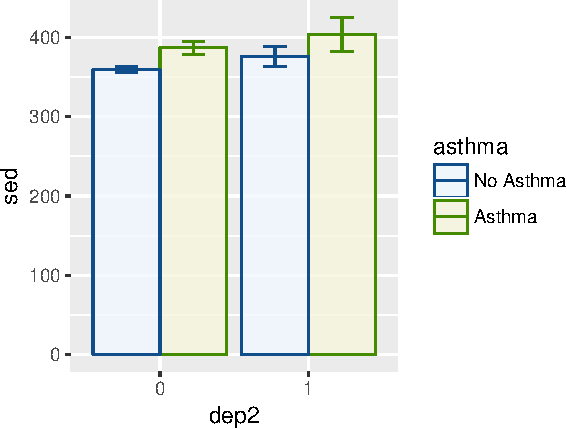
\includegraphics{09_AdvancedPlotting_files/figure-beamer/cs1-1.pdf}

\end{frame}

\begin{frame}[fragile]{Color Schemes}

Just so you are aware:

\begin{itemize}
\tightlist
\item
  aliceblue is a lightblue
\item
  beige is a light green
\item
  dodgerblue4 is a dark blue
\item
  chartreuse4 is a dark green
\end{itemize}

So the \texttt{fill} colors are light and the \texttt{color} colors are
dark in this example. You, of course, can do whatever you want
color-wise. I'm a fan of this style though so we will keep it for now.

These same functions can be used on the other plots as well. Feel free
to give them a try. As for the book, we'll move on to the next section:
Themes.

\end{frame}

\section{Themes}\label{themes}

\begin{frame}[fragile]{Themes}

Using the plot we just made--the bar plot--we will show how theme
options work. There are several built in themes that change many aspects
of the plot (e.g., \texttt{theme\_bw()}, \texttt{theme\_classic()},
\texttt{theme\_minimal()}). There are many more if you download the
\texttt{ggthemes} package. Fairly simply you can create plots similar to
those in newspapers and magazines.

\end{frame}

\begin{frame}[fragile]{Themes}

First, we are going to save the plot to simply show the different
theming options.

\begin{Shaded}
\begin{Highlighting}[]
\NormalTok{p =}\StringTok{ }\KeywordTok{position_dodge}\NormalTok{(}\DataTypeTok{width =}\NormalTok{ .}\DecValTok{9}\NormalTok{)}
\NormalTok{p1 =}\StringTok{ }\KeywordTok{ggplot}\NormalTok{(summed_data, }\KeywordTok{aes}\NormalTok{(}\DataTypeTok{x =}\NormalTok{ dep2, }\DataTypeTok{y =}\NormalTok{ sed, }
                             \DataTypeTok{group =}\NormalTok{ asthma)) }\OperatorTok{+}
\StringTok{  }\KeywordTok{geom_bar}\NormalTok{(}\KeywordTok{aes}\NormalTok{(}\DataTypeTok{fill =}\NormalTok{ asthma, }\DataTypeTok{color =}\NormalTok{ asthma), }
           \DataTypeTok{stat =} \StringTok{"identity"}\NormalTok{, }
           \DataTypeTok{position =}\NormalTok{ p,}
           \DataTypeTok{alpha =}\NormalTok{ .}\DecValTok{8}\NormalTok{) }\OperatorTok{+}
\StringTok{  }\KeywordTok{geom_errorbar}\NormalTok{(}\KeywordTok{aes}\NormalTok{(}\DataTypeTok{ymin =}\NormalTok{ sed }\OperatorTok{-}\StringTok{ }\NormalTok{s_se, }\DataTypeTok{ymax =}\NormalTok{ sed }\OperatorTok{+}\StringTok{ }\NormalTok{s_se,}
                    \DataTypeTok{color =}\NormalTok{ asthma), }
                \DataTypeTok{position =}\NormalTok{ p,}
                \DataTypeTok{width =}\NormalTok{ .}\DecValTok{3}\NormalTok{) }\OperatorTok{+}
\StringTok{  }\KeywordTok{scale_color_manual}\NormalTok{(}\DataTypeTok{values =} \KeywordTok{c}\NormalTok{(}\StringTok{"dodgerblue4"}\NormalTok{, }
                                \StringTok{"chartreuse4"}\NormalTok{)) }\OperatorTok{+}\StringTok{  }
\StringTok{  }\KeywordTok{scale_fill_manual}\NormalTok{(}\DataTypeTok{values =} \KeywordTok{c}\NormalTok{(}\StringTok{"aliceblue"}\NormalTok{, }\StringTok{"beige"}\NormalTok{))}
\end{Highlighting}
\end{Shaded}

\end{frame}

\begin{frame}[fragile]{Theme Black and White}

\begin{Shaded}
\begin{Highlighting}[]
\NormalTok{p1 }\OperatorTok{+}\StringTok{ }
\StringTok{  }\KeywordTok{theme_bw}\NormalTok{()}
\end{Highlighting}
\end{Shaded}

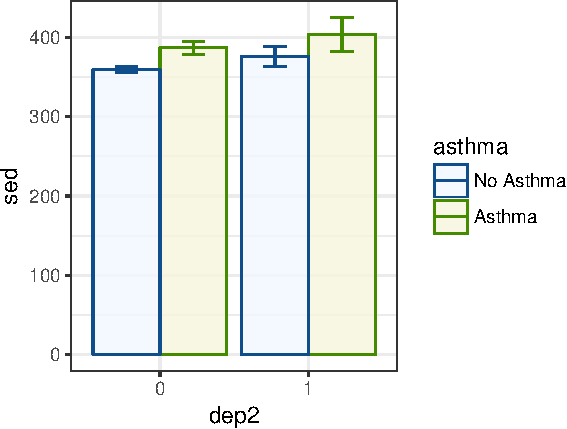
\includegraphics{09_AdvancedPlotting_files/figure-beamer/unnamed-chunk-6-1.pdf}

\end{frame}

\begin{frame}[fragile]{Theme Classic}

\begin{Shaded}
\begin{Highlighting}[]
\NormalTok{p1 }\OperatorTok{+}\StringTok{ }
\StringTok{  }\KeywordTok{theme_classic}\NormalTok{()}
\end{Highlighting}
\end{Shaded}

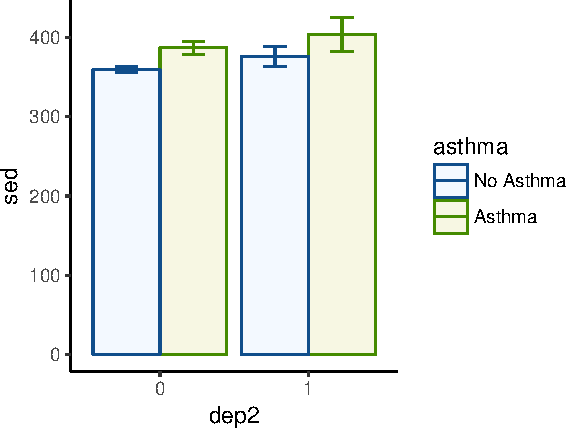
\includegraphics{09_AdvancedPlotting_files/figure-beamer/unnamed-chunk-7-1.pdf}

\end{frame}

\begin{frame}[fragile]{Theme Minimal}

\begin{Shaded}
\begin{Highlighting}[]
\NormalTok{p1 }\OperatorTok{+}\StringTok{ }
\StringTok{  }\KeywordTok{theme_minimal}\NormalTok{()}
\end{Highlighting}
\end{Shaded}

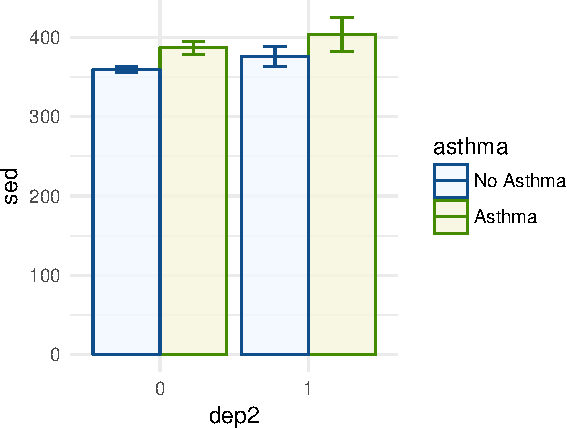
\includegraphics{09_AdvancedPlotting_files/figure-beamer/unnamed-chunk-8-1.pdf}

\end{frame}

\begin{frame}[fragile]{Theme Economist (from \texttt{ggthemes})}

\begin{Shaded}
\begin{Highlighting}[]
\KeywordTok{library}\NormalTok{(ggthemes)}
\NormalTok{p1 }\OperatorTok{+}\StringTok{ }
\StringTok{  }\KeywordTok{theme_economist}\NormalTok{()}
\end{Highlighting}
\end{Shaded}

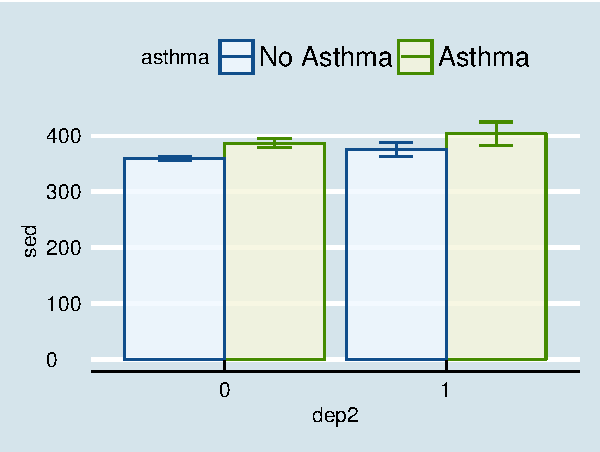
\includegraphics{09_AdvancedPlotting_files/figure-beamer/unnamed-chunk-9-1.pdf}

\end{frame}

\begin{frame}[fragile]{Theme FiveThirtyEight (from \texttt{ggthemes})}

\begin{Shaded}
\begin{Highlighting}[]
\NormalTok{p1 }\OperatorTok{+}\StringTok{ }
\StringTok{  }\KeywordTok{theme_fivethirtyeight}\NormalTok{()}
\end{Highlighting}
\end{Shaded}

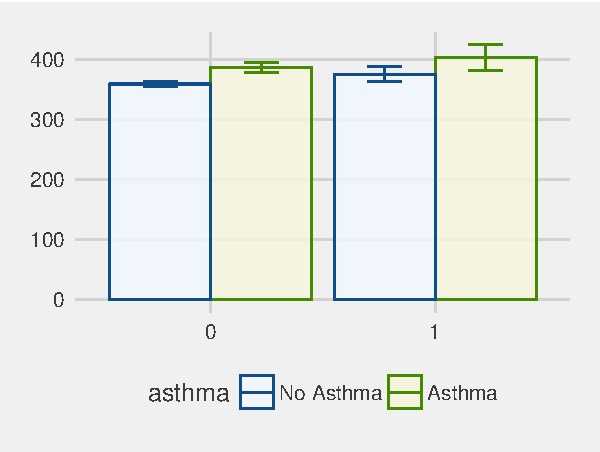
\includegraphics{09_AdvancedPlotting_files/figure-beamer/unnamed-chunk-10-1.pdf}

\end{frame}

\begin{frame}[fragile]{Theme Tufte (from \texttt{ggthemes})}

\begin{Shaded}
\begin{Highlighting}[]
\NormalTok{p1 }\OperatorTok{+}\StringTok{ }
\StringTok{  }\KeywordTok{theme_tufte}\NormalTok{()}
\end{Highlighting}
\end{Shaded}

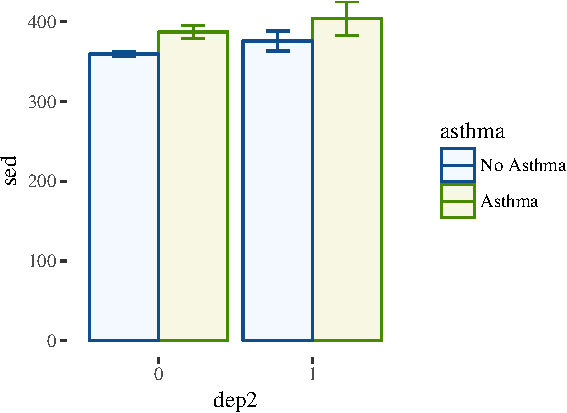
\includegraphics{09_AdvancedPlotting_files/figure-beamer/unnamed-chunk-11-1.pdf}

\end{frame}

\begin{frame}[fragile]{Your Own Theme}

There are many more but you get the idea. In addition to the built in
themes, you can use the \texttt{theme()} function and make your own
adjustments. There are \emph{many} options so we will just introduce the
idea.

\begin{Shaded}
\begin{Highlighting}[]
\NormalTok{p1 }\OperatorTok{+}\StringTok{ }
\StringTok{  }\KeywordTok{theme}\NormalTok{(}\DataTypeTok{legend.position =} \StringTok{"bottom"}\NormalTok{,  }
        \DataTypeTok{legend.background =} \KeywordTok{element_rect}\NormalTok{(}\DataTypeTok{color =} \StringTok{"lightgrey"}\NormalTok{),}
        \DataTypeTok{panel.background =} \KeywordTok{element_rect}\NormalTok{(}\DataTypeTok{fill =} \StringTok{"grey99"}\NormalTok{, }
                                        \DataTypeTok{color =} \StringTok{"grey70"}\NormalTok{), }
        \DataTypeTok{text =} \KeywordTok{element_text}\NormalTok{(}\DataTypeTok{family =} \StringTok{"Times"}\NormalTok{))  }
\end{Highlighting}
\end{Shaded}

\end{frame}

\begin{frame}{Your Own Theme}

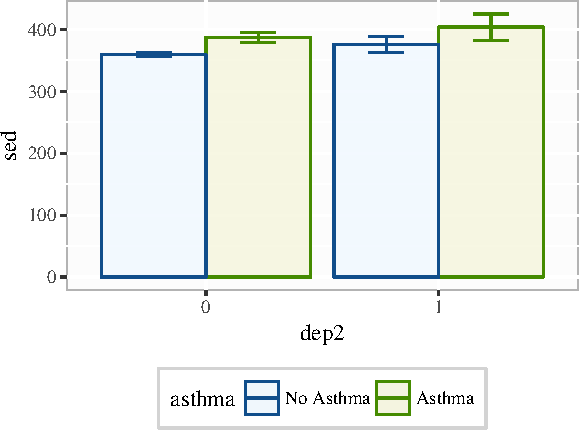
\includegraphics{09_AdvancedPlotting_files/figure-beamer/t1-1.pdf}

There are many more options but essentially if there is something you
want to change, you probably can.

\end{frame}

\section{Labels and Titles}\label{labels-and-titles}

\begin{frame}[fragile]{Labels and Titles}

Using our last plot, we will also want to add good labels and/or titles.

\begin{Shaded}
\begin{Highlighting}[]
\NormalTok{p1 }\OperatorTok{+}\StringTok{ }
\StringTok{  }\KeywordTok{theme}\NormalTok{(}\DataTypeTok{legend.position =} \StringTok{"bottom"}\NormalTok{,  }
        \DataTypeTok{legend.background =} \KeywordTok{element_rect}\NormalTok{(}\DataTypeTok{color =} \StringTok{"lightgrey"}\NormalTok{),}
        \DataTypeTok{panel.background =} \KeywordTok{element_rect}\NormalTok{(}\DataTypeTok{fill =} \StringTok{"grey99"}\NormalTok{,}
                                        \DataTypeTok{color =} \StringTok{"grey70"}\NormalTok{),}
        \DataTypeTok{text =} \KeywordTok{element_text}\NormalTok{(}\DataTypeTok{family =} \StringTok{"Times"}\NormalTok{)) }\OperatorTok{+}
\StringTok{  }\KeywordTok{labs}\NormalTok{(}\DataTypeTok{y =} \StringTok{"Sedentary Behavior (Minutes)"}\NormalTok{,}
       \DataTypeTok{x =} \StringTok{"Depression (1 = Depressed)"}\NormalTok{,}
       \DataTypeTok{title =} \StringTok{"Comparison of Sedentary Behavior"}\NormalTok{,}
       \DataTypeTok{subtitle =} \StringTok{"across Depression and Asthma"}\NormalTok{)}
\end{Highlighting}
\end{Shaded}

\end{frame}

\begin{frame}{Labels and Titles}

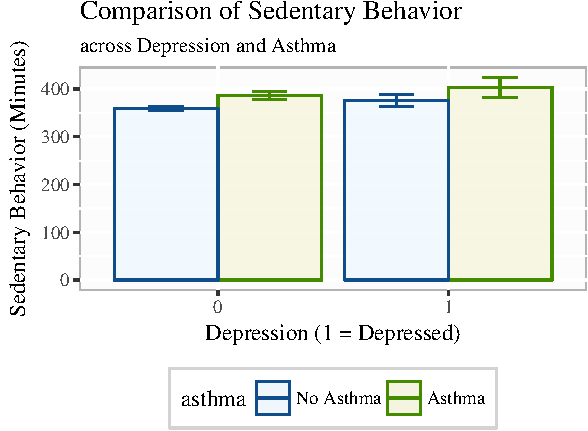
\includegraphics{09_AdvancedPlotting_files/figure-beamer/l1-1.pdf}

\end{frame}

\section{Facetting}\label{facetting}

\begin{frame}[fragile]{Facetting}

Facetting is very useful when trying to compare more than three
variables at a time or you cannot use color or shading. It is often
useful and beautiful. Facetting splits the data based on some grouping
variable (e.g., asthma) to highlight differences in the relationship.

\begin{Shaded}
\begin{Highlighting}[]
\NormalTok{p1 }\OperatorTok{+}\StringTok{ }
\StringTok{  }\KeywordTok{theme}\NormalTok{(}\DataTypeTok{legend.position =} \StringTok{"bottom"}\NormalTok{,  }
        \DataTypeTok{legend.background =} \KeywordTok{element_rect}\NormalTok{(}\DataTypeTok{color =} \StringTok{"lightgrey"}\NormalTok{),}
        \DataTypeTok{panel.background =} \KeywordTok{element_rect}\NormalTok{(}\DataTypeTok{fill =} \StringTok{"grey99"}\NormalTok{,}
                                        \DataTypeTok{color =} \StringTok{"grey70"}\NormalTok{),}
        \DataTypeTok{text =} \KeywordTok{element_text}\NormalTok{(}\DataTypeTok{family =} \StringTok{"Times"}\NormalTok{)) }\OperatorTok{+}
\StringTok{  }\KeywordTok{labs}\NormalTok{(}\DataTypeTok{y =} \StringTok{"Sedentary Behavior (Minutes)"}\NormalTok{,}
       \DataTypeTok{x =} \StringTok{"Depression (1 = Depressed)"}\NormalTok{,}
       \DataTypeTok{title =} \StringTok{"Comparison of Sedentary Behavior"}\NormalTok{,}
       \DataTypeTok{subtitle =} \StringTok{"across Depression and Asthma"}\NormalTok{) }\OperatorTok{+}
\StringTok{  }\KeywordTok{facet_grid}\NormalTok{(}\OperatorTok{~}\NormalTok{asthma)}
\end{Highlighting}
\end{Shaded}

\end{frame}

\begin{frame}{Facetting}

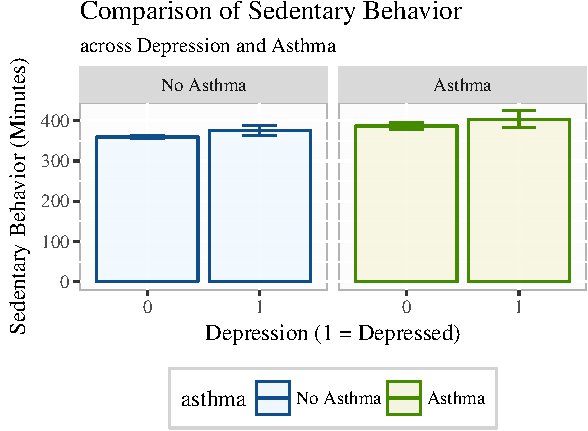
\includegraphics{09_AdvancedPlotting_files/figure-beamer/f1-1.pdf}

You can facet by more than one variable and it will create separate
panels for each combination of the facetting variables.

\end{frame}

\section{Conclusions}\label{conclusions}

\begin{frame}[fragile]{Conclusions}

This was a quick, but deeper, demonstration of plotting with
\texttt{ggplot2}. There is so much more you can do.

However, in the end, exploring and communicating the data through plots
is simply something you need to practice. With time, you can \emph{a
priori} picture the types of plots that will highlight things in your
data, the ways you can adjust it, and how you need to manipulate your
data to make it plot ready.

Be patient and have fun trying things. In my experience, almost anytime
I think, ``Can R do this?'', it can, so try to do cool stuff and you'll
probably find that you can.

\end{frame}
